% !TeX root = ../Thesis.tex

%************************************************
\chapter{Evaluation and Results}
\label{evaluation}
%************************************************
%\glsresetall % Resets all acronyms to not used
This section provides a comprehensive assessment and analysis of the middleware’s performance utilizing defined performance metrics of throughput and response time, custom workload, and custom benchmarking process. The middleware’s performance is evaluated across various test scenarios, featuring different middleware configurations based on the performance metrics introduced in the subsection \ref{performanceMetrics}. The performance with and without the middleware using the same workloads are compared applying the experimental setup and methodology outlined in the subsection \ref{setupMethod}. \\

\noindent Subsequently, the subsection \ref{throughputAnalysis} examines the impacts of configuration changes of the middleware on average throughput and average response time. From the generated test results, the average throughput and the average response time of the middleware are derived. Moreover, the results from the performance analysis are interpreted and investigated to identify anticipated bottlenecks and limitations in the middleware, and potential solutions for optimization are suggested. \\

\noindent Finally, the subsection \ref{throughputAnalysis} provides a brief overview of the nearly balanced data distribution among the Redis databases achieved through the middleware’s consistent hash sharding approach. 

%***************************************************************************
%***************************************************************************
\section{Performance Metrics}
\label{performanceMetrics}

\begin{figure}[H]
             \ffigbox{
\includegraphics[scale = 0.45]{gfx/figures/Baseline_Response_Latency.pdf}}{\caption[Illustration of latency, processing time and response time observed in baseline]{Illustration of latency, processing time and response time measured in the baseline for comparison}\label{latency_response_baseline}}
\end{figure}

\textbf{Latency} is the time duration between the initiation of a request transmission by a source and the reception of the corresponding message by the destination. Such latency manifests as the time in which the request is held in a waiting state prior to processing. Round-trip latency, whereas, is defined as time elapsed between the transmission of a request and the receipt of the corresponding response. It does not account for the processing time incurred at the destination. In the system architecture examined in this thesis, two types of latency require consideration. The first latency type involves round-trip latency occurring throughout the communication between the client and the middleware, while the second type pertains to round-trip latency in the interaction between the middleware and the associated Redis database instances. Both latencies are crucial for comprehending the overall performance of the proposed middleware and are measured in milliseconds (ms). \\

\noindent \textbf{Processing time} refers to the time taken by a processing system to execute a received request. It is computed as the time duration between the moment when the system receives the final byte of the request and the moment when it transmits the first byte of response. To evaluate the performance of the proposed system of sharded distributed databases, the processing time for all operations performed by the middleware is assessed. These processing times enclose the time taken for decomposing requests from the client into multiple sub-requests, sharding associated data and allocating it to appropriate Redis database, constructing pipelines to transmit the sub-requests to appropriate shards, merging the received partial results from the involved Redis databases and aggregating these partial results to generate a corresponding response to the initial request. The processing time for the middleware is measured in milliseconds (ms). \\

\noindent \textbf{Response time} of the examined system is the total time elapsed from the initiation of a request transmission to the receipt of the corresponding response, measured in milliseconds (ms). It represents a cumulative time duration, comprising both the latency and internal processing time of the entire system. For the evaluation, two average response times are measured. The first measurement, i.e., the average response time of the baseline, is obtained from the client-side when connected directly to a single Redis database without the middleware. The second measurement is the average response time observed from the client when connected to the middleware. Comparing these average response times provides valuable insights into the performance impact of the middleware on the system. \\

\noindent \textbf{Throughput} is a performance metric, which quantifies the total number of requests that a system can successfully process within a given time. In the context of this evaluation, the middleware’s throughput is thoroughly examined, as it is responsible for handling all incoming client requests. The middleware’s throughput is expressed in Requests Per Second (RPS). Factors influencing the throughput of the middleware include computing resources of the host machine on which the middleware is installed, the processing overhead associated with the middleware, the degree of parallelism or concurrency within the middleware and the types of requests the middleware processes. To facilitate a comparison, the average throughput of the baseline, i.e., a single Redis database employing the same workload as the middleware, is measured.
The workload employed for evaluating response time and throughput is interpreted in the subsection \ref{workloadBenchmark}. \\

\noindent The observed latencies, processing times, and response times in the baseline for comparison are illustrated in \cref{latency_response_baseline}, while those for the middleware-assisted sharded distributed databases are depicted in \cref{latency_response}.

\begin{figure}[H]
             \ffigbox{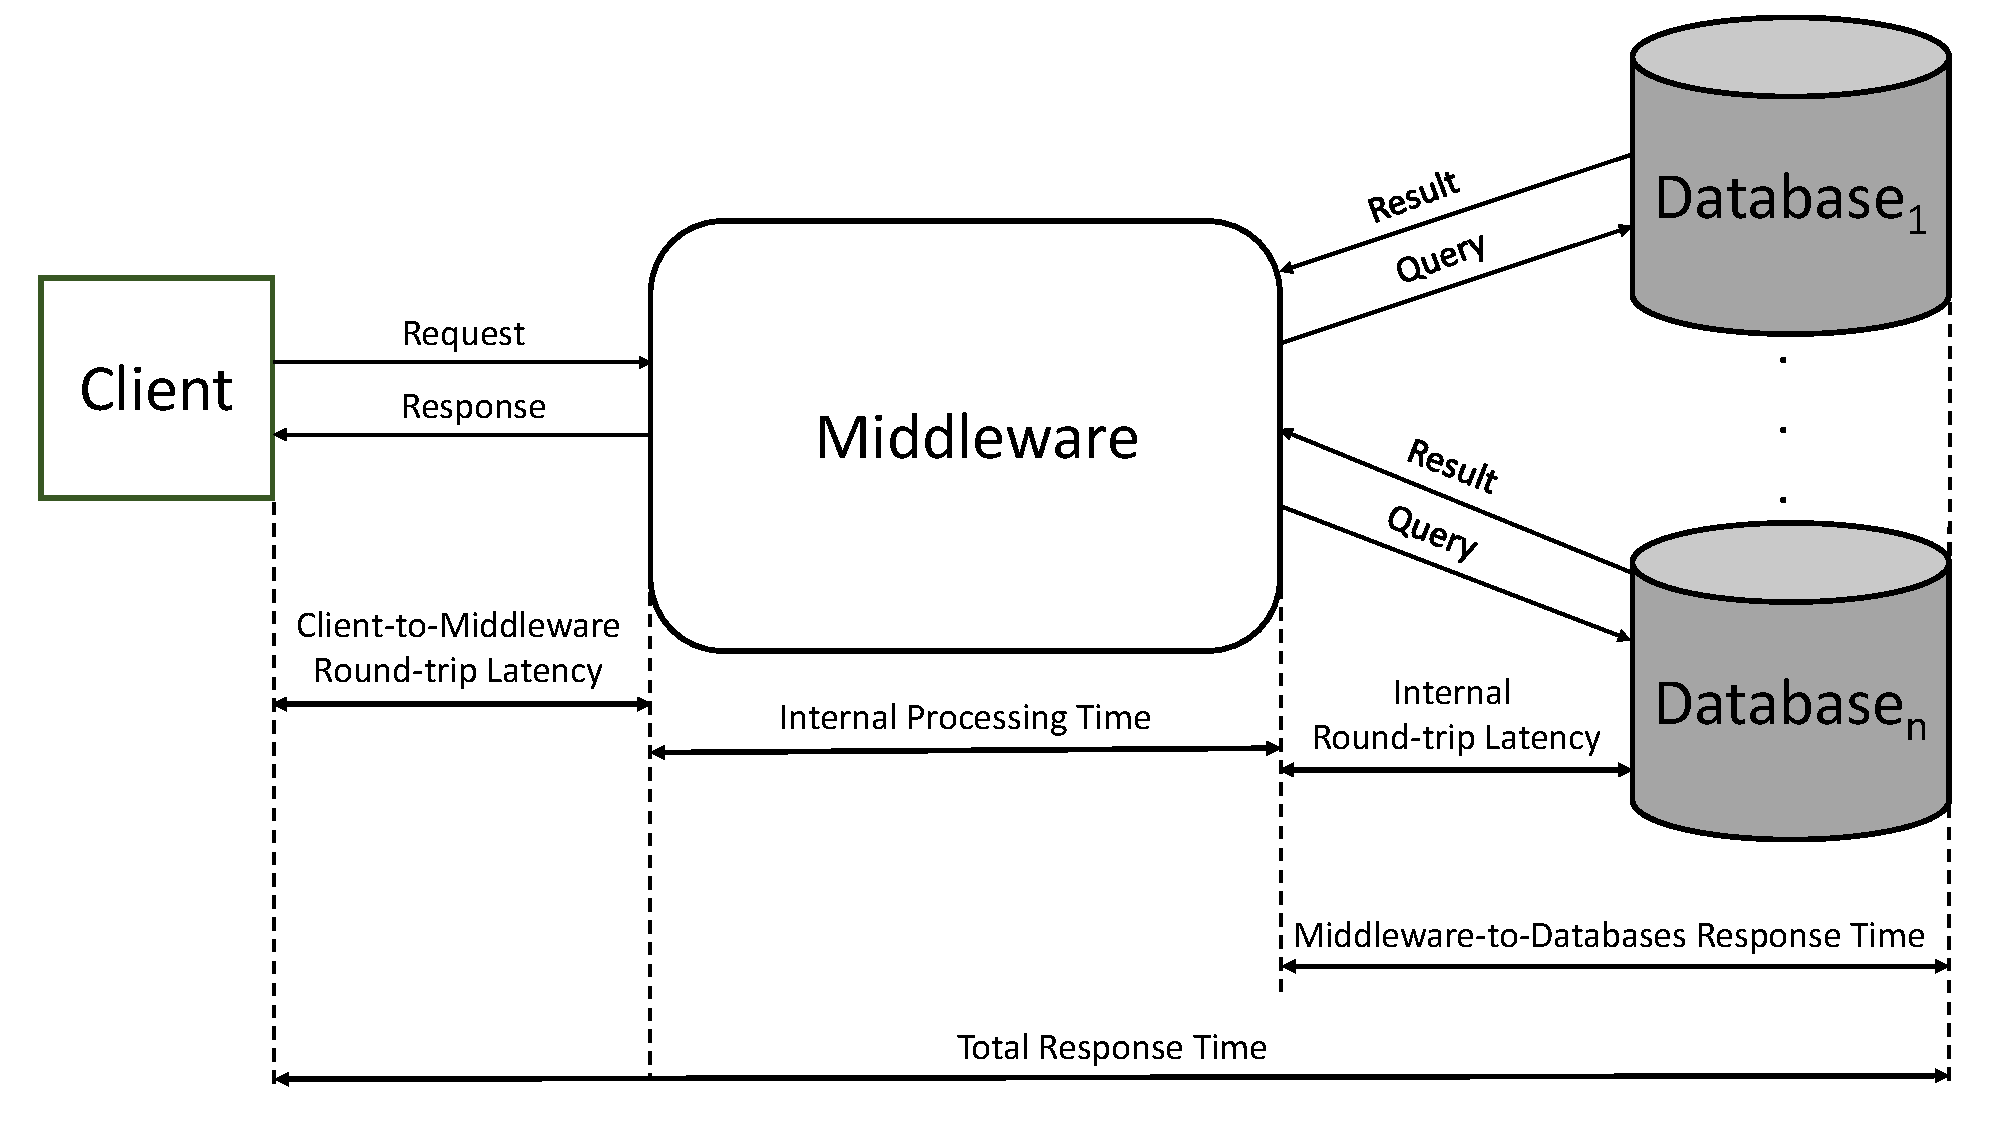
\includegraphics[scale = 0.45]{gfx/figures/Latency_Response_M.pdf}}{\caption[Illustration of observed latencies, processing time and response times in middleware-assisted sharded distributed databases]{Comprehensive illustration of latencies, processing time and response times measured in the proposed system of middleware-assisted sharded distributed databases}\label{latency_response}}
\end{figure}

%\begin{figure}[H]
%             \ffigbox{
\includegraphics[scale = 0.45]{gfx/reports/Report_3_18_2023_4_19_pm.pdf}}{\caption{Performance evaluation of the middleware through benchmarking, where a load of 100 concurrent clients are generated progressively at the rate of 10 clients per second}\label{benchmark}}
%\end{figure}
%%%%%%%%%%%%%%%%%%%%%%%
\begin{comment}   
\begin{figure}[H]
	\begin{floatrow}
             \ffigbox{
\includegraphics[scale = 0.5]{gfx/visualizations/set.pdf}}{\caption{Set Key-Value Pairs}\label{set}}
             \ffigbox{
\includegraphics[scale = 0.5]{gfx/visualizations/get.pdf}}{\caption{Get Key-Value Pairs}\label{get}}
	\end{floatrow}
\end{figure}
\begin{figure}[H]
	\begin{floatrow}
             \ffigbox{
\includegraphics[scale = 0.5]{gfx/visualizations/get-range.pdf}}{\caption{Get Range Of Key-Value Pairs}\label{getRange}}
             \ffigbox{
\includegraphics[scale = 0.5]{gfx/visualizations/delete.pdf}}{\caption{Delete Key-Value Pairs}\label{delete}}
	\end{floatrow}
\end{figure}

\begin{figure}[H]
             \ffigbox{
\includegraphics[width=\textwidth]{gfx/visualizations/combined_visualization.pdf}}{\caption{Average response time per given key-value pairs of all functions provided by middleware}\label{combined}}
\end{figure}

\end{comment}
%%%%%%%%%%%%%%%%%%%%%%%

%***************************************************************************
%***************************************************************************
\section{Experimental Setup and Methodology}
\label{setupMethod}
In this subsection custom workload and benchmarking process are devised to conduct tests with concrete configurations and evaluate the middleware’s performance across different test scenarios.

%***************************************************************************
%***************************************************************************
\subsection{Custom Workload and Benchmarking Process}
\label{workloadBenchmark}
This study uses a custom workload consisting of two distinct datasets, $Dataset_{1}$ and $Dataset_{2}$, to evaluate the performance of the middleware-assisted sharded distributed databases. $Dataset_{1}$, the larger of the two, comprises 1000 key-value pairs, whereas the smaller dataset, $Dataset_{2}$ contains 100 key-value pairs. Each key within these datasets is a randomly generated 4-digit integer, which is associated with a value holding 3 distinct key-value pairs. The associated values consist of the key identifiers: $UserID$, $Name$, and $Email$. Among these key identifiers, $UserID$ serves as the shard key. The schema used in the datasets is exemplified with \cref{key-value-schema}. \\

\begin{figure}[H]
             \ffigbox{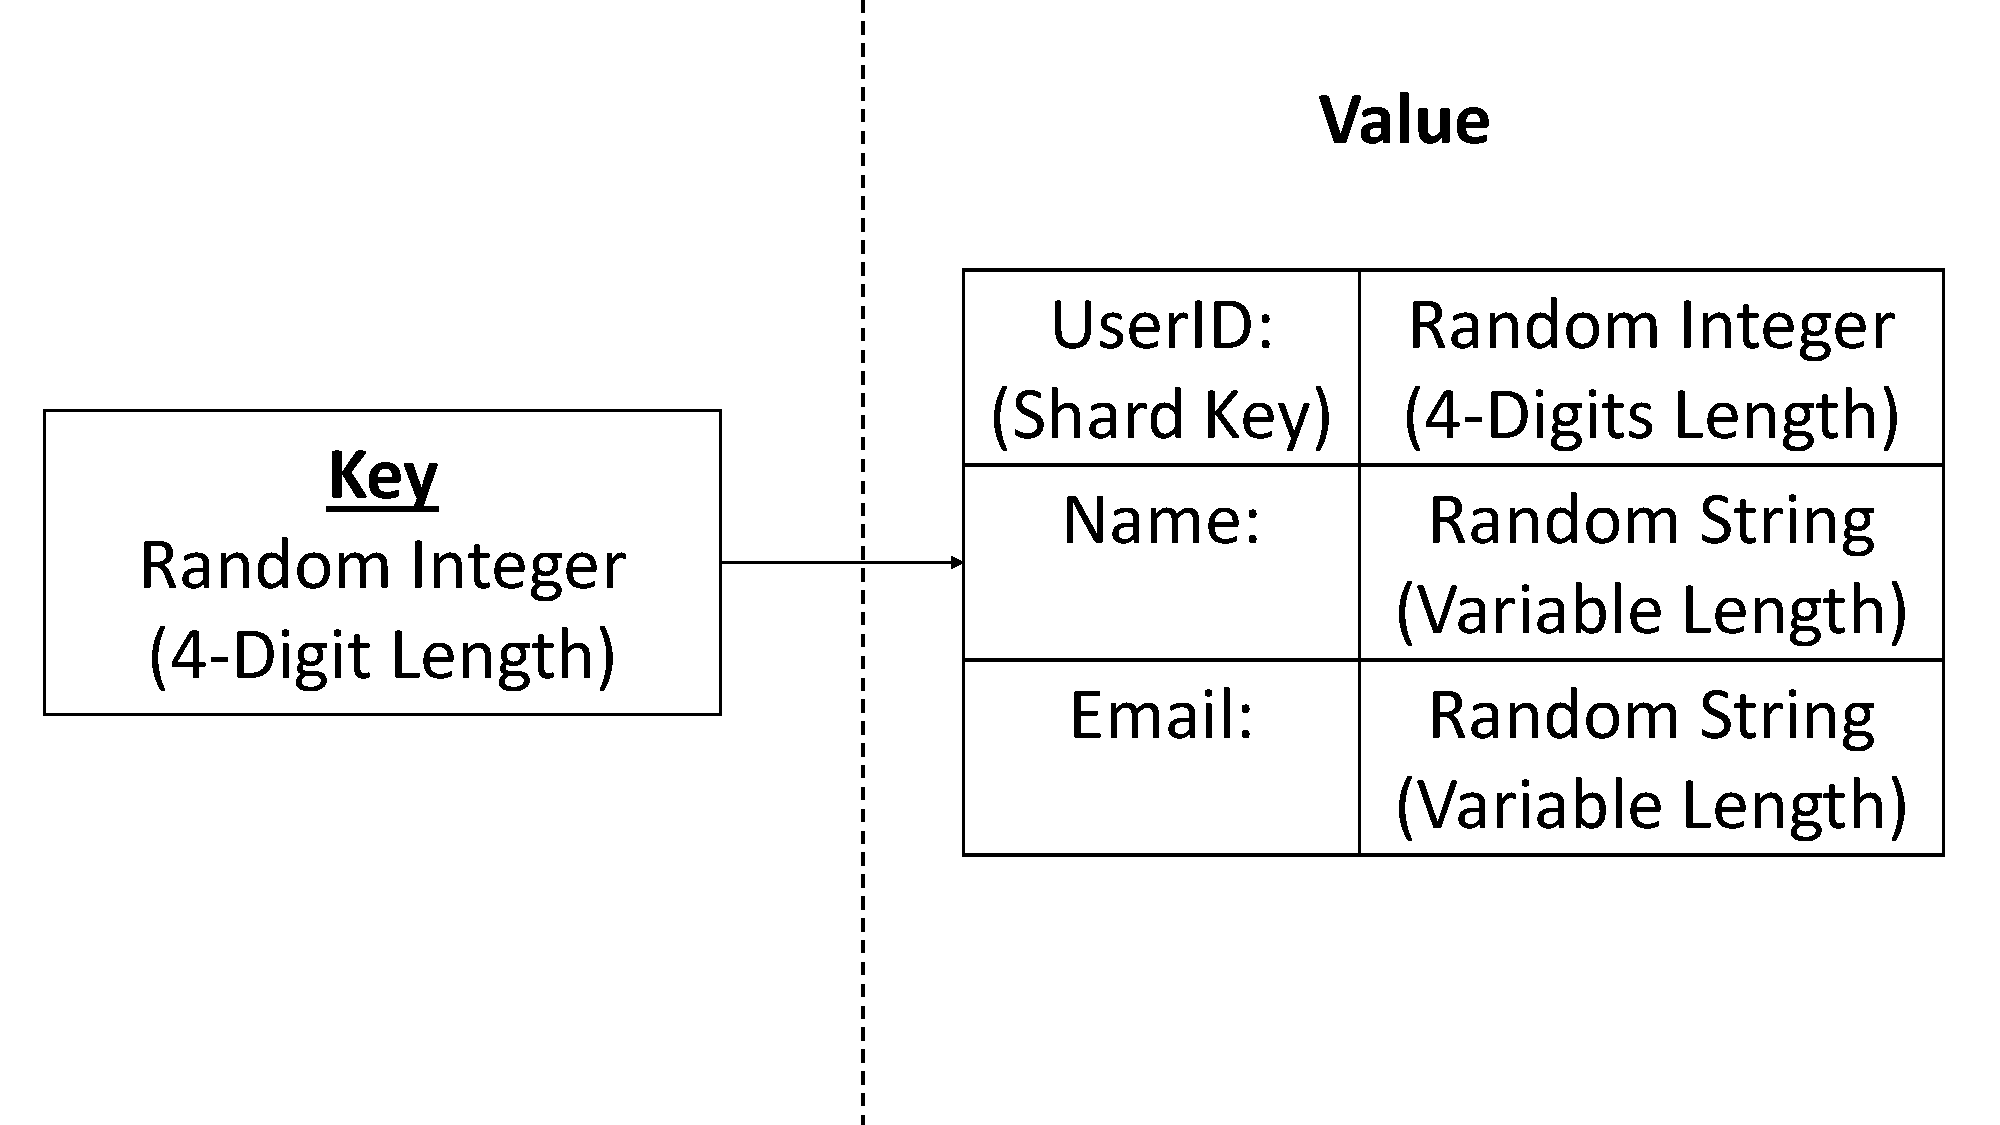
\includegraphics[scale = 0.25]{gfx/figures/workload_schema.pdf}}{\caption{Workload Schema}\label{key-value-schema}}
\end{figure}

\noindent    The custom benchmarking process evaluates the performance of various operations supported by the middleware using both $Dataset_{1}$ and $Dataset_{2}$. All operations use either single or multiple key-value pairs. To differentiate between the two, $Dataset_{1}$ is used for $set$, $get$, $get$-$range$, and $delete$ operations involving multiple key-value pairs, while $Dataset_{2}$ is used for $set$ and $get$ operations with single key-value pair. To simulate real-world scenarios with read-heavy and write-heavy operations, all 1000 key-value pairs from $Dataset_{1}$ are used for $set$ and $get$ operations with multiples key-value pairs. In contrast, only 100 keys are used for $get$-$range$ and $delete$ operations. For $set$, $get$, and $delete$ operations with single key-value pair, 1 randomly chosen key-value pair from $Dataset_{2}$ is employed. \\

\noindent \cref{tab:workload} presents a breakdown of the workload distribution for evaluating all specified operations of the middleware.
%You can find an example table in \cref{tab:workload} using the \emph{tabular} environment. Note the use of horizontal lines from the \emph{booktabs} package (\lstinline|\toprule|, \lstinline|\midrule|, and \lstinline|\bottomrule|) and removed whitespace at both sides of the table (\lstinline|@{}|) as proposed by Markus Püschel.\footnote{\url{https://www.inf.ethz.ch/personal/markusp/teaching/guides/guide-tables.pdf}}
%
\begin{table} [H]
\centering
\begin{tabular}{@{} lccr @{}} % @{} removes white spaces
	\toprule
	\tableheadlineL{Operations} & \tableheadline{Requests} & \tableheadline{Dataset} & \tableheadlineR{Tested Workload} \\ 
	\midrule
	\multirow{2}{*}{set} & set\textunderscore single & Dataset\textsubscript{2} & 1 Key-Value Pair \\
		& set\textunderscore multiple & Dataset\textsubscript{1} & 1000 Key-Value Pairs \\
	 \midrule
	\multirow{2}{*}{get} & get\textunderscore single & Dataset\textsubscript{2} & 1 Key-Value Pair \\
		& get\textunderscore multiple & Dataset\textsubscript{1} & 1000 Key-Value Pairs \\
	 \midrule
	get-range & get\textunderscore range & Dataset\textsubscript{1} & 100 Key-Value Pairs \\
	\midrule
	\multirow{2}{*}{delete} & del\textunderscore single & Dataset\textsubscript{2} & 1 Key-Value Pair \\
		& del\textunderscore multiple & Dataset\textsubscript{1} & 100 Key-Value Pair \\
	\bottomrule
\end{tabular}
% Use alternative short title for table of contents with \caption [SHORT-TITLE]
\caption{Workload distribution for tested operations}
\label{tab:workload}
\end{table}

\noindent To evaluate the middleware's average throughput and average response time, Locust  framework, a Python-based open-source load-testing tool, is utilized \cite{locust}. This tool simulates load of numerous concurrent clients on System Under Test (SUT), facilitating the analysis of the system’s behavior when subjected to high traffic from multiple concurrent clients. The load-testing is conducted under two distinct contexts. The initial context involves executing all operations directly on a single Redis database without the middleware, serving as the baseline configuration. This configuration adheres to the specified workload for the operations, as outlined in \cref{tab:workload}. In the subsequent context, the client is connected to the middleware, having different configurations as detailed in the subsection \ref{config}. In this context, all the operations with specified workload from \cref{tab:workload} are tested to gain insights about the middleware’s performance. \\

\noindent The middleware uses the Python module, \emph{logging} for generating internal logs and insights to measure the average processing time within the middleware and to determine the internal response time of connected Redis database instances to the middleware \cite{logging}. The \emph{timeit} Python module is used to estimate the execution time of the middleware for each operation over 1 million iterations \cite{timeit}. The return value is the average execution time in seconds. To measure the internal response time from the associated Redis databases within the middleware, the \emph{time.time()} function from the Python in-built module \emph{time} is used. This function returns the time since the Unix epoch, as a floating-point number expressed in seconds \cite{time}. For the custom benchmarking in this thesis, all values from the logs are converted to milliseconds (ms).


%***************************************************************************
%***************************************************************************
\subsection{System Configuration}
\label{config}
The middleware, the core component of the proposed sharded distributed databases, is the System Under Test (SUT). Every test scenario for performance evaluation is composed of one instance of middleware connected with varying number of Redis database instances. The number of client instances depends upon the test scenario. \\

\noindent The middleware and the Redis databases, used for the performance analysis are installed on separate machines, each with following specifications:
\begin{itemize}
\item[-] Processor: Intel(R) Xeon(R) Silver 4214R CPU @ 2.40GHz (24 CPU cores)
\item[-]  Memory: 32 GiB RAM
\item[-]  Operating System: Ubuntu 22.04.1 LTS
\end{itemize}
In contrast, each client machine is equipped with the following specifications:
\begin{itemize}
\item[-]  Processor: Intel(R) Core (TM) i5-9400F CPU @2.90GHz (6 CPU cores)
\item[-]  Memory: 8GiB RAM
\item[-]  Operating System: Windows 11 Home 64 bit
\end{itemize}

\noindent For testing and evaluation of the SUT, different parameters are considered, which are as follows:
\begin{itemize}
\item \textbf{Workload:} $Dataset_{1}$ and $Dataset_{2}$ as described in the subsection \ref{workloadBenchmark}. 
\item \textbf{Client-load:} It is the number of concurrent clients performing all operations ($set$, $get$, $get$-$range$, and $delete$) involving single and multiple key-value pairs. Depending upon the test scenario, the client-load remains constant or increases gradually with time throughout the test execution.
\item \textbf{Baseline:} It is the configuration where the client connects directly with 1 Redis database and performs all given operations without the middleware. It serves as a starting point for comparing and analyzing the performance of the middleware. The baseline tests are executed with the custom workload, $Dataset_{1}$ and $Dataset_{2}$.
\end{itemize}

\noindent To obtain an in-depth evaluation of the middleware’s performance, four different configurations regarding the number of connected Redis databases and shards are considered. Each middleware’s configuration is tested separately to facilitate a clear comparison. To diminish further complexities in the middleware’s configurations, multiple shards within a database are disregarded and each database instance is treated as a single shard. The middleware is consequently subjected to the following configurations during the load test:
\begin{itemize}
\item \textbf{M:1 -} 1 middleware instance connected with 1 Redis database node (1 shard).
\item \textbf{M:2 -} 1 middleware instance connected with 2 Redis database nodes (2 shards).
\item \textbf{M:4 -} 1 middleware instance connected with 4 Redis database nodes (4 shards).
\item \textbf{M:6 -} 1 middleware instance connected with 6 Redis database nodes (6 shards).
\end{itemize}


%***************************************************************************
%***************************************************************************
\subsection{Test Scenario}
\label{testScenario}
Using the aforementioned configurations of the middleware in the subsection \ref{config}, two distinct conditions are applied for the load testing process aiming to measure the performance of the middleware in terms of average throughput and average response time. The applied test conditions are as follows: \\

\begin{enumerate}

\item \textbf{Constant client-load for each load-test execution:} \\

\noindent In this case, a consistent number of clients is maintained throughout the testing process of each testing scenario. Each test scenario encompasses a baseline configuration and all middleware configurations (M:1, M:2, M:4, and M:6). There are in total 3 test scenarios and each is subjected to a constant client-load of 1, 10, and 100 respectively. An overview of these test scenarios is illustrated in \cref{constant-client-load}.

\begin{figure}[H]
             \ffigbox{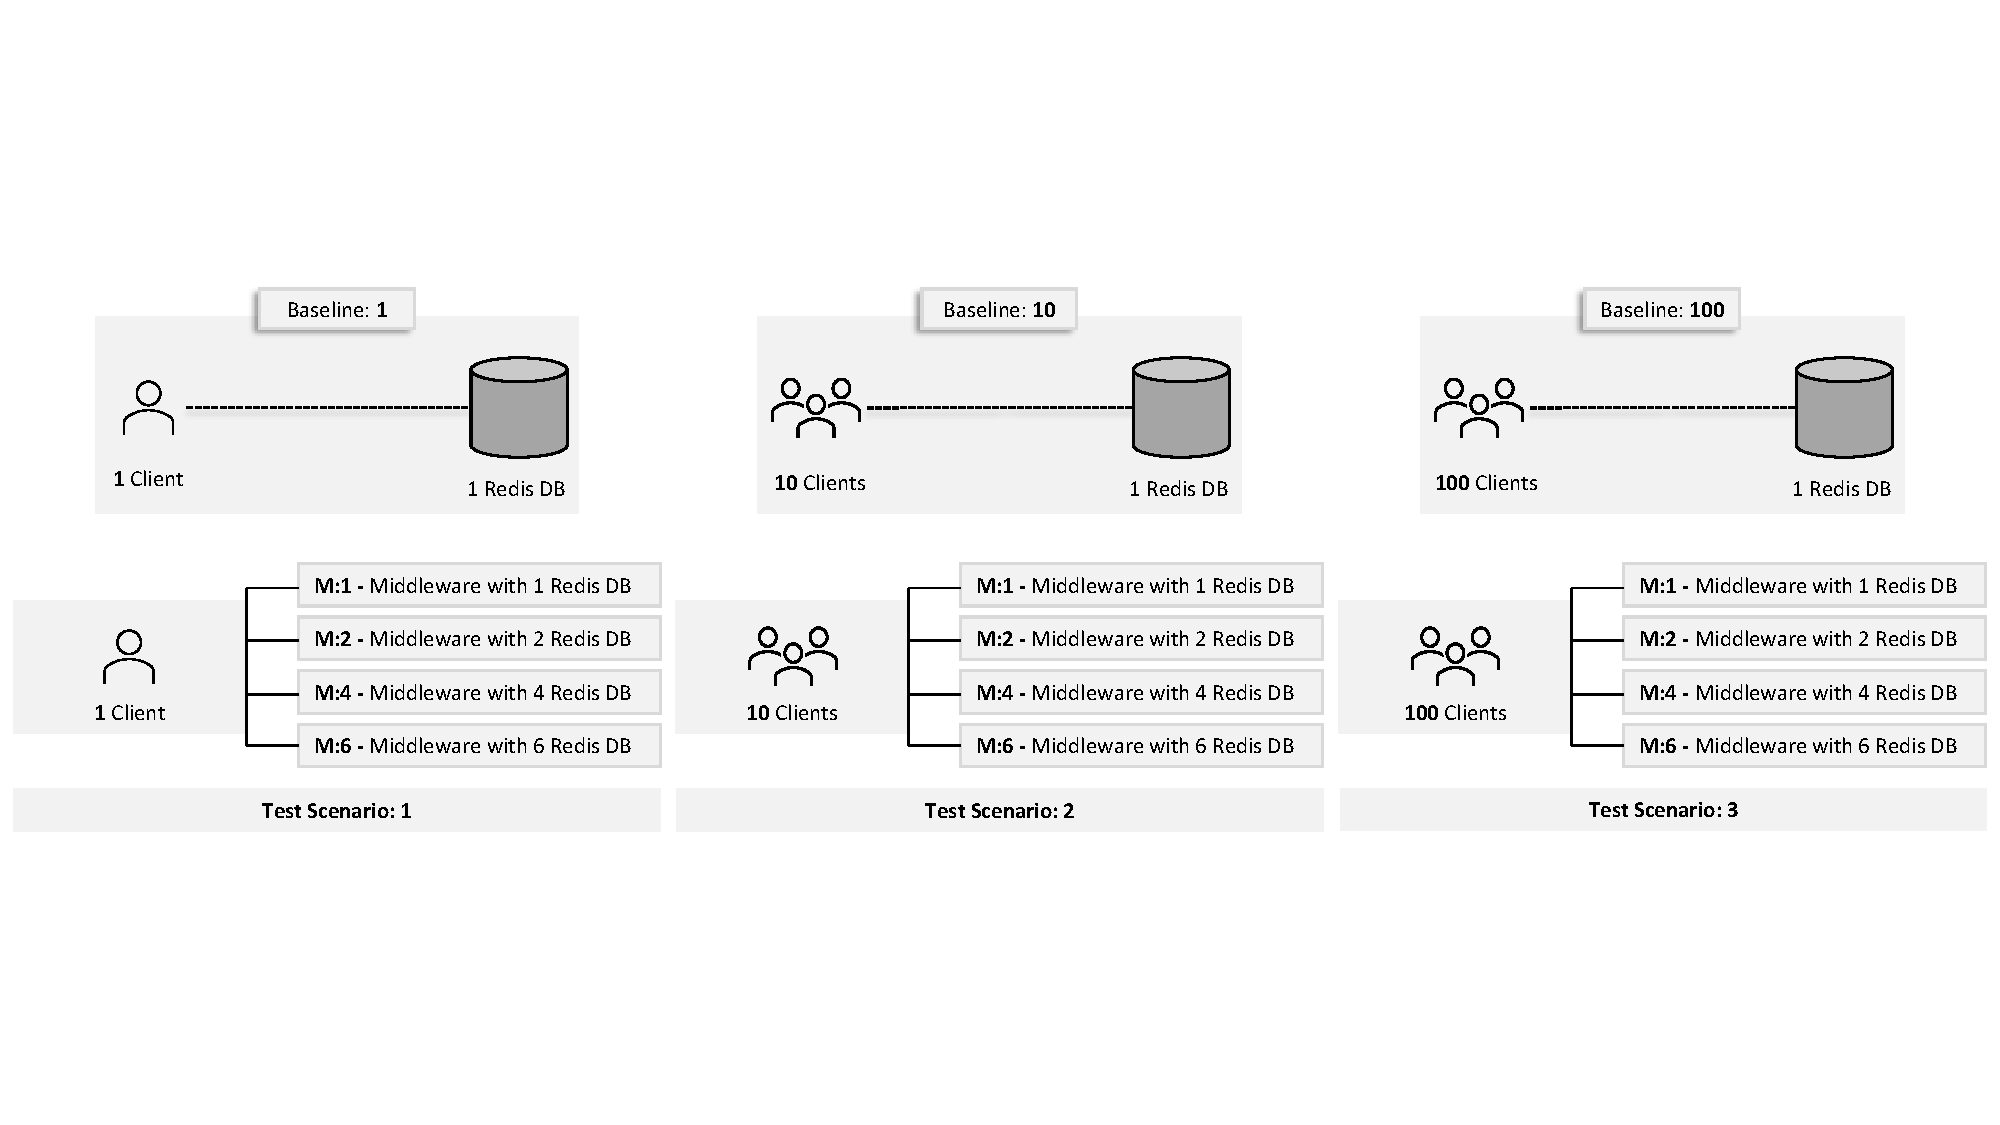
\includegraphics[width=\textwidth]{gfx/figures/Test_Scenario_Constant_Client_Load.pdf}}{\caption[Test scenarios for constant client-load]{Illustration of all test scenarios to measure and compare average throughput and average response time of the middleware relative to baseline and taking client-load variation into account for each scenario; DB: Database}\label{constant-client-load}}
\end{figure}

This approach assists in a more straightforward comparison of the impact that varying number of connected Redis databases to the middleware has on the performance under a constant workload over time. Moreover, this approach identifies the level of the client-load that causes the middleware to be overloaded and determines whether the middleware can handle additional clients. \\

\item \textbf{Gradually increasing client-load for the load-test execution:} \\

\noindent In this test condition, the client-load progressively increases throughout the load-testing phase for the baseline and for each middleware configuration. The number of clients, i.e., client-load starting with 1 client, grows at a spawning rate of 1 client every 2 seconds until a saturation point is reached. For the performance evaluation in this thesis, a maximum limit of 50 concurrent clients is considered for this test scenario. A visual representation of the test scenario under this specific condition is depicted in \cref{increasing-client-load}.

\begin{figure}[H]
             \ffigbox{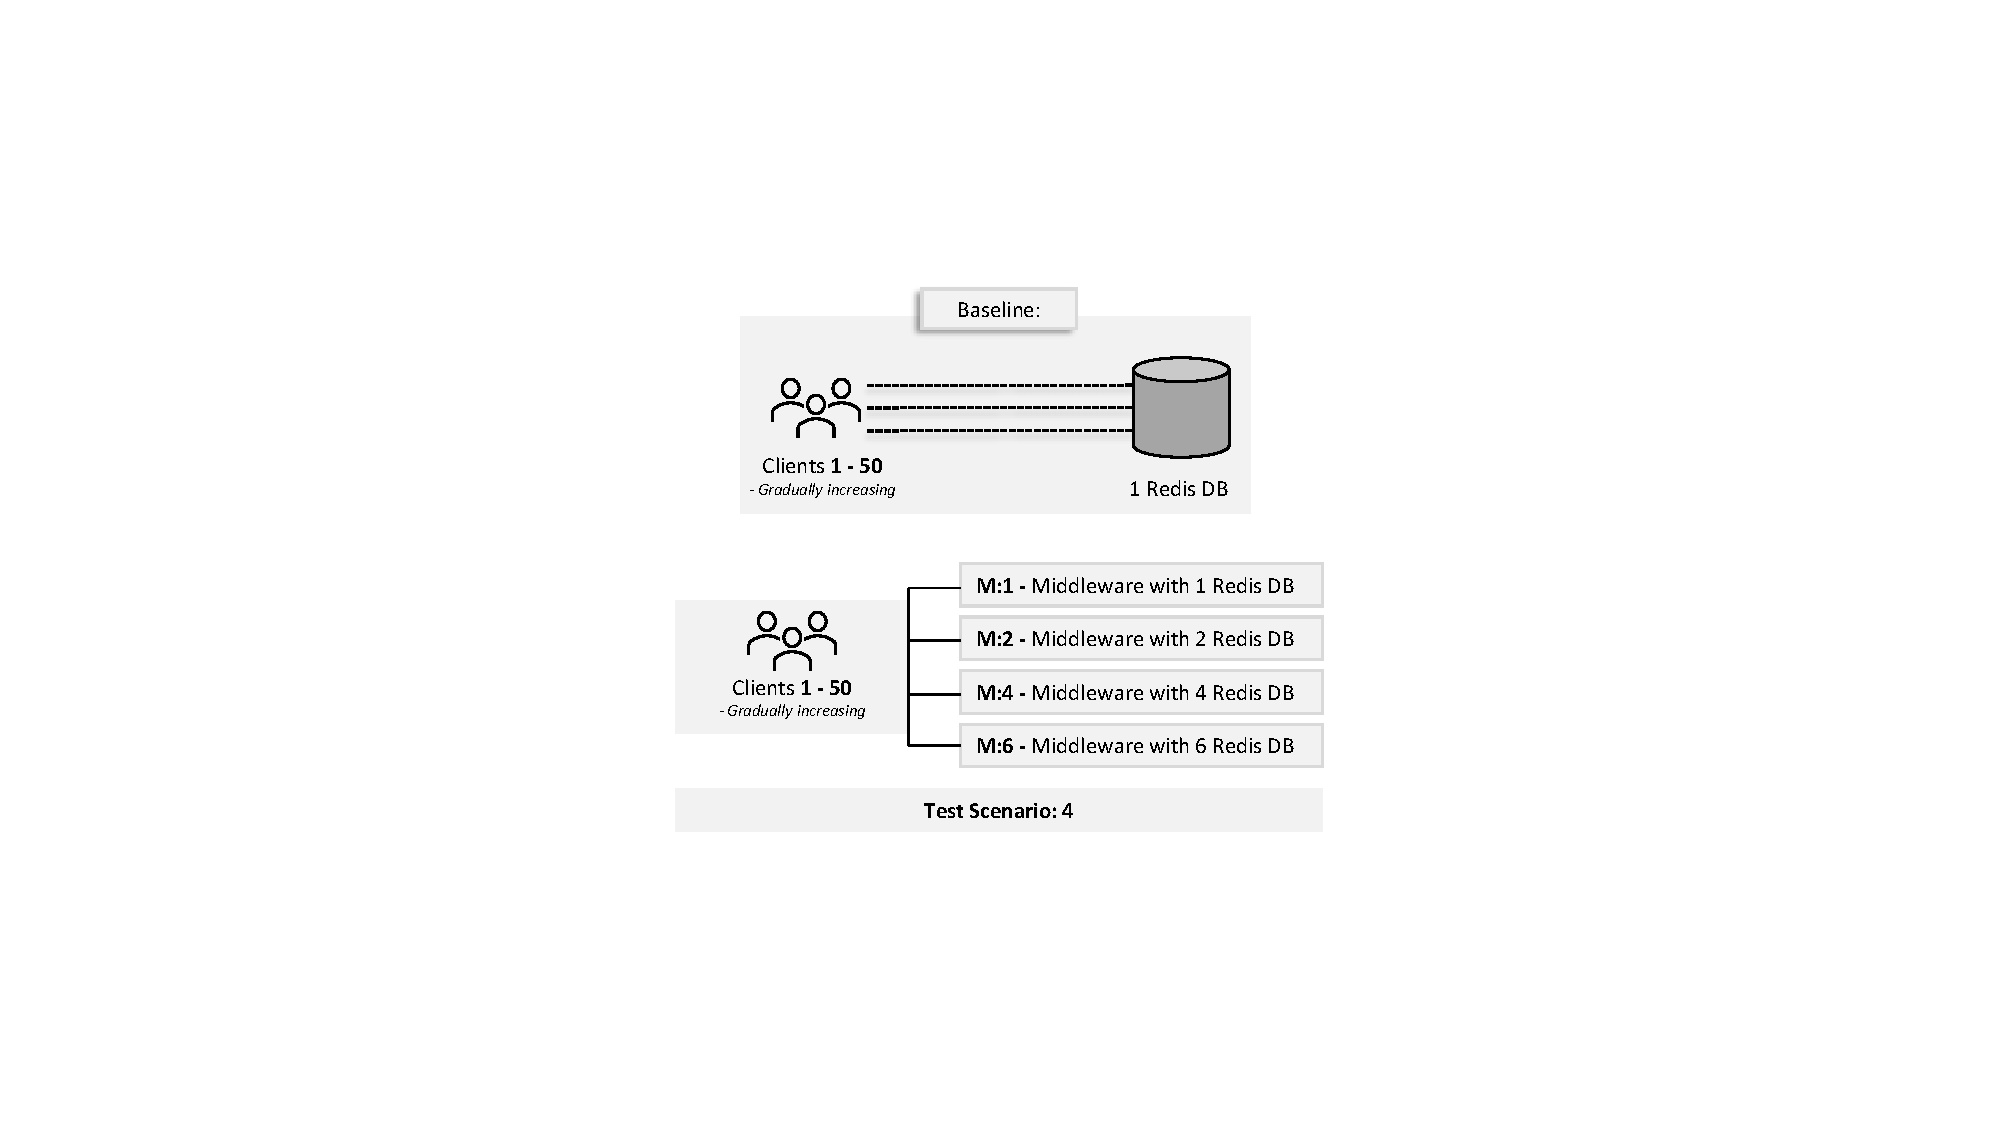
\includegraphics[width=\textwidth]{gfx/figures/Test_Scenario_Varying_Client_Load.pdf}}{\caption[Test scenarios for increasing client-load]{Illustration of test scenario with gradually increasing clients to measure and compare average throughput and response time of the middleware across different configurations, relative to baseline}\label{increasing-client-load}}
\end{figure}

\end{enumerate}


%***************************************************************************
%***************************************************************************
\section{Throughput and Response Time Analysis}
\label{throughputAnalysis}

Building upon the test conditions and the test scenarios defined in the subsection \ref{testScenario}, the performance of the middleware with respect to the established baseline, specifically in terms of average throughput and average response time, is analyzed and evaluated in this subsection. 

%***************************************************************************
%***************************************************************************
\subsection*{\textbf{Average Throughput}}

In the constant client-load condition, there are 3 test scenarios (Test Scenario: 1, Test Scenario: 2, and Test Scenario: 3) as illustrated in the \cref{constant-client-load}. The load-test execution for each test scenario with constant client-load is conducted for 3 minutes using the middleware configurations from the subsection \ref{config}. A warm-up time and cool-down time of 10 seconds each are excluded from the test execution time, accounting for system startup, process initialization, garbage collection, and system teardown. From the remaining 2 minutes and 40 seconds, only the test execution period of 1 minute is considered, where the system reaches a stable state. \\

\noindent In each test scenario, a baseline is established, where the client is connected to 1 Redis database and performs all the operations from the \cref{tab:workload}. All the operations are performed using the workloads $Dataset_{1}$ and $Dataset_{2}$ as defined in the subsection \ref{workloadBenchmark}. The custom workload is ready-heavy and write-heavy, resembling most real-world scenarios. The middleware’s behavior, when connected with 1, 2, 4, and 6 Redis databases, is evaluated in relation to the corresponding baseline for each scenario. For each client-load situation, the workload remains the same, i.e., all clients perform all operations using the same key-value pairs. This approach ensures that the middleware can handle all operations on identical key-value pairs. \\

%%%%%%%%%%%%
\noindent In \textbf{Test Scenario: 1} with a constant client-load of 1, the baseline's average throughput observed during the test execution ranges from approximately 95 to 100 Requests per Second (RPS). The findings also imply that the client’s average throughput, when operating with the middleware, remains stable between 45 and 60 RPS throughout the 1 minute of test execution, as depicted in the \cref{throughput_1_client}. \\

\begin{figure}[H]
             \ffigbox{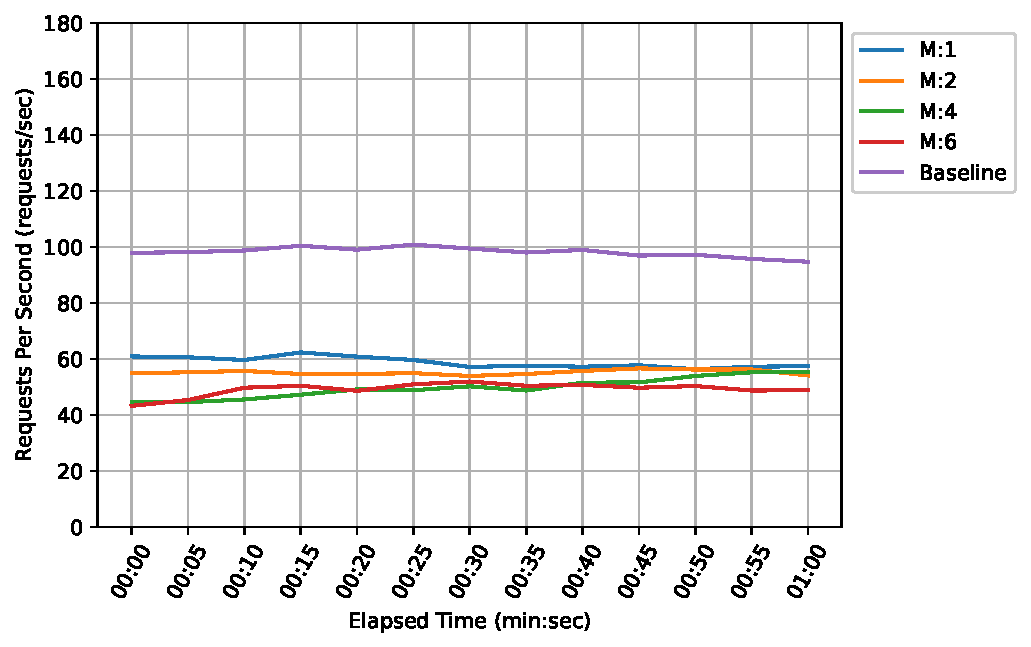
\includegraphics[width=\textwidth]{gfx/reports/throughput/throughput(rps)_1_Client.pdf}}{\caption{Average throughput measurement with 1 client-load (Test Scenario: 1)}\label{throughput_1_client}}
\end{figure}

\noindent When the middleware connected to 1 Redis database, the average throughput is around 58.4 RPS, which is marginally higher than other middleware configurations. However, when connected to 2 Redis databases, the average throughput of the middleware decreases to 53.7 RPS. This trend persists, with the middleware connected to 4 Redis databases exhibiting an average throughput of 50.6 RPS, and the middleware connected to 6 Redis databases yielding approximately 48.2 RPS. This clearly demonstrates that the throughput of the middleware connected to 1 Redis database (M:1) can handle approximately 10 more requests than that of the middleware connected to 6 Redis databases (M:6). \\

%%%%%%%%%%%%
\noindent In \textbf{Test Scenario: 2}, featuring a constant client-load of 10, the difference in observed throughput between the middleware with different configurations and the baseline remains consistent with the results observed under a client-load of 1. However, there is an increase in the middleware’s throughput as the client-load increases. This suggests that the middleware with a client-load of 1 is not saturated enough and can accommodate more concurrent clients. With the increased client-load of 10, the middleware can handle approximately 20 requests more every second than with the client-load of 1. Across all middleware configurations, the average throughput ranges from 70 to 75 RPS. But the trend for the middleware configurations, where additional Redis databases result in slightly lower throughput, persists in this case as well. The baseline’s average throughput in this case reaches approximately 153 RPS, which is a substantial difference from the prior test scenario. Likewise, the middleware demonstrates improved performance compared to the previous test scenario. However, the baseline configuration still facilitates higher throughput, as shown in the \cref{throughput_10_client}. \\

\begin{figure}[H]
             \ffigbox{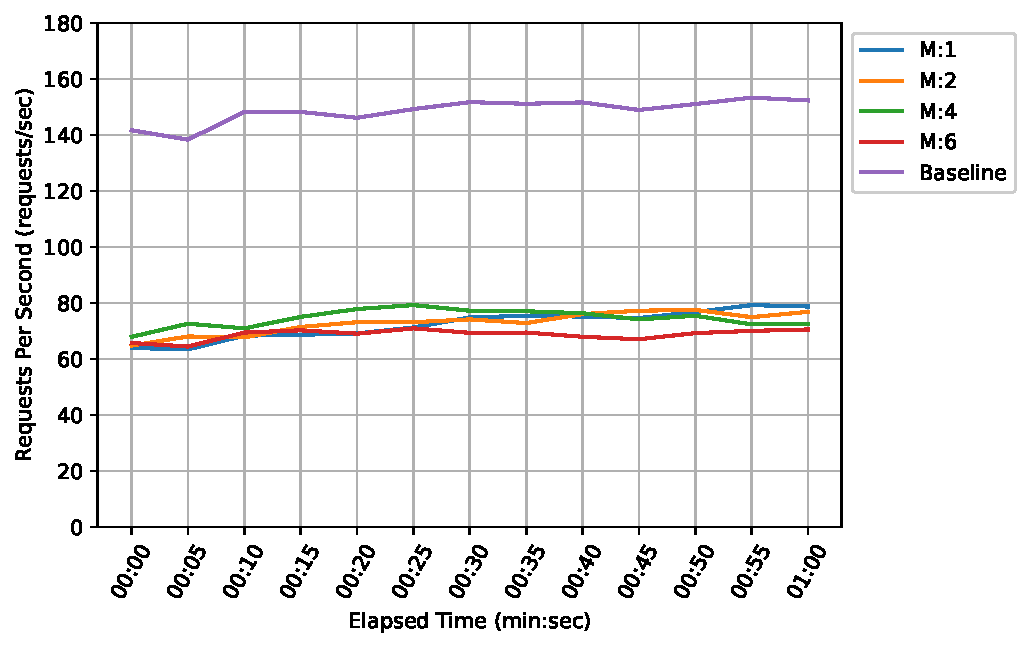
\includegraphics[width=\textwidth]{gfx/reports/throughput/throughput(rps)_10_Client.pdf}}{\caption{Average throughput measurement with 10 client-load (Test Scenario: 2)}\label{throughput_10_client}}
\end{figure}

\noindent In \textbf{Test Scenario: 3} with the client-load of 100, the average throughput of the baseline increases up to 170 RPS before starting to decrease, ultimately reaching around 160 RPS. This indicates that the baseline has reached its saturation point, with its computing resources being fully utilized. This is presumably due to the inability of 1 Redis database to handle the requests from 100 concurrent clients and execute operations with the same workload simultaneously. A deeper investigation of this behavior falls outside the scope of this thesis. However, the average throughput of all middleware configurations remains consistent at around 70 to 80 RPS, indicating that the middleware is saturated at this point. One of the potential reasons for the lack of throughput increase in the middleware could be potential increase in the response times, which will be discussed together with the evaluation of average response time.  \\

\noindent \cref{throughput_100_client} illustrates the variation of the middleware’s average throughput for each configuration with the client-load of 100, referencing to the baseline. \\

\begin{figure}[H]
             \ffigbox{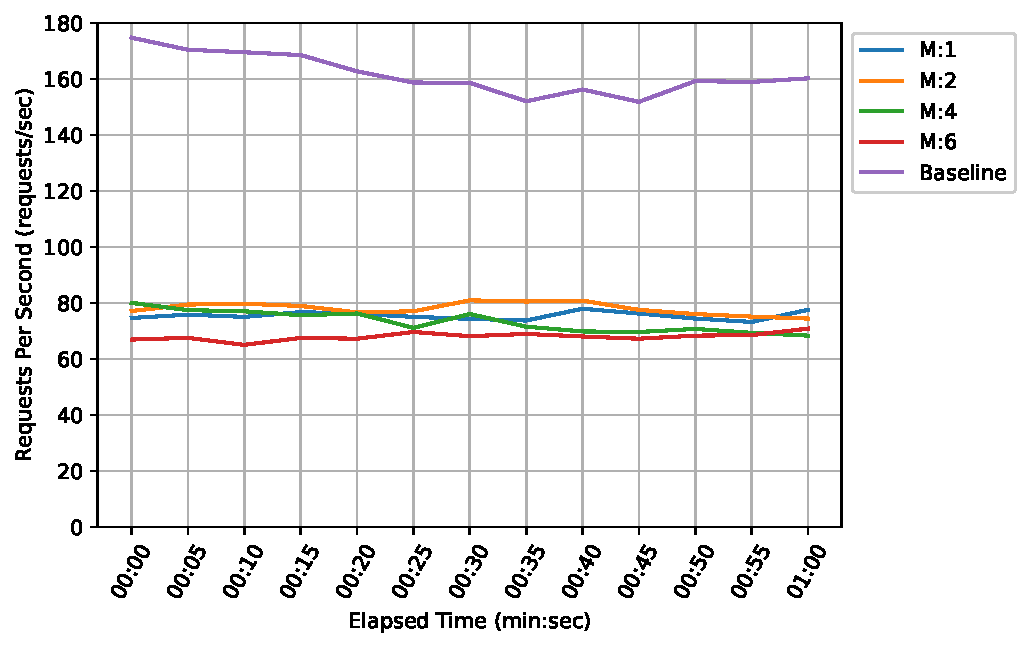
\includegraphics[width=\textwidth]{gfx/reports/throughput/throughput(rps)_100_Client.pdf}}{\caption{Average throughput measurement with 100 client-load (Test Scenario: 3)}\label{throughput_100_client}}
\end{figure}

\noindent \cref{tab:summary_constant_client} provides a summary of the average throughput of the baseline and the middleware observed in each given test scenario. The middleware’s throughput saturation point is at around 70 RPS from the given results. The average throughput initially increases and subsequently stabilizes when all the computing resources of the middleware are occupied. As the middleware is fully engaged in executing the operations for the corresponding requests, it becomes congested at a point and cannot accommodate more requests. \\

\begin{table} [H]
\centering
\begin{tabular}{@{} lcrrrrr @{}} % @{} removes white spaces
	\toprule
	Test Scenario & Client-load	&	Baseline	&	M:1	&	M:2  &		M:4  & 	M:6  \\
	%\tableheadlineL{Test} & \tableheadline{Client} & \tableheadline{Baseline} & \multirow{2}{*}{\spacedlowsmallcaps{M:1}} &  \multirow{2}{*}{\spacedlowsmallcaps{M:2}} &  \multirow{2}{*}{\spacedlowsmallcaps{M:4}} &  \multirow{2}{*}{\spacedlowsmallcaps{M:6}} \\ 
	%\tableheadlineL{Scenario}& \tableheadline{(N)*} & \tableheadline{(N)} & &  &  &  \\ 
	\midrule
	1	&	1 &	94.9 RPS	&	58.4 RPS	&	53.7 RPS	&	50.6 RPS	&	48.2 RPS \\
	2	&	10 &	153.0 RPS	&	76.3 RPS	&	74.6 RPS	&	71.5 RPS	&	70.7 RPS \\
	3	&	100 &	161.2 RPS	&	74.6 RPS	&	73.4 RPS	&	71.3 RPS	&	70.7 RPS \\
	\bottomrule
\end{tabular}
\caption[Average throughput measured during load-test execution with constant client-loads]{Average throughput measured during load-test execution with constant client-loads; Client-load*}
\label{tab:summary_constant_client}
\end{table}

\noindent An insightful evaluation of the middleware’s average throughput involves a comparison of its performance with gradually increasing client-load, which is defined as \textbf{Test Scenario: 4} in the subsection \ref{testScenario}. An overview of the observed results from the load-test execution of increasing client-load from 1 to 50 at a steady rate of 1 client every 2 seconds is shown in \cref{average_rps_50}. The outcomes in this test scenario are comparable to those in the test scenarios with constant client-load. \\

\begin{figure}[H]
             \ffigbox{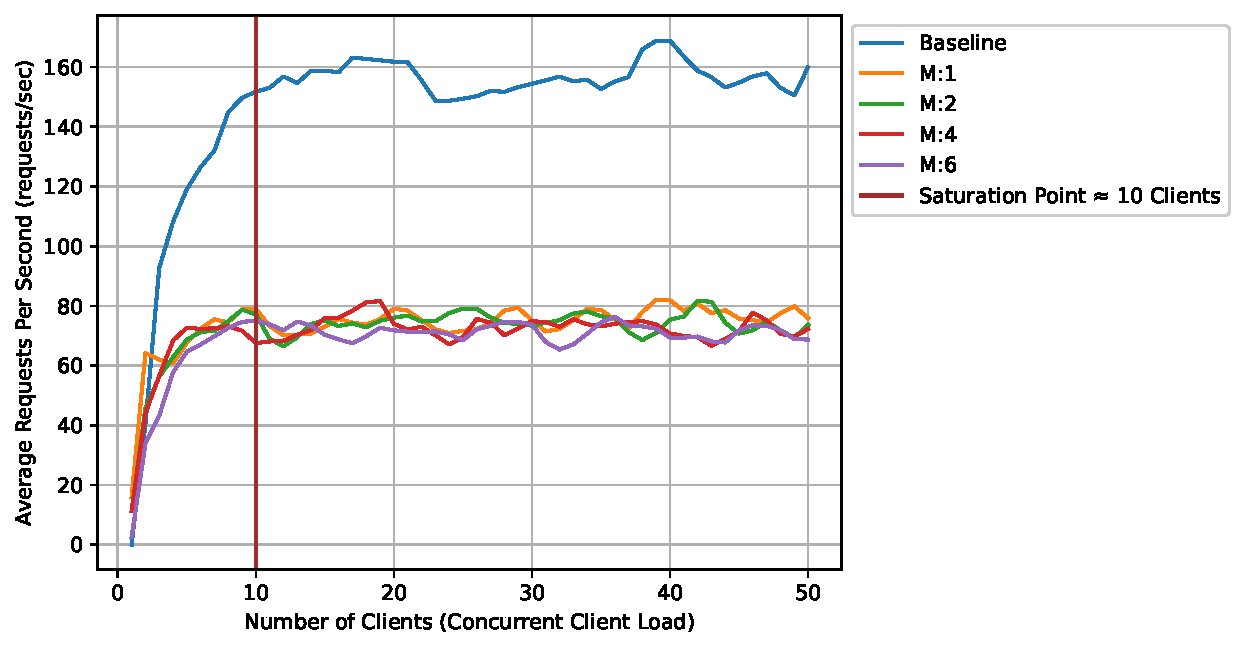
\includegraphics[width=\textwidth]{gfx/reports/throughput/average_rps_50.pdf}}{\caption{Average throughput with respect to increasing client-load ranging from 1 to 50 (Test Scenario: 4)}\label{average_rps_50}}
\end{figure}

\noindent The baseline without the middleware, i.e., the single Redis database, does not exhibit a stable and significant increase in the average throughput beyond the client-load of 10. From that point, the average throughput fluctuates and becomes unstable. Similarly, for the middleware with different configurations of the Redis databases, the average throughput increases with an increasing number of clients to 10. However, there is no notable improvement in average throughput beyond the client-load of 10. This suggests that both the baseline and the middleware with different configurations can be evaluated with the client-load ranging from 1 to 10, with 10 being the approximate saturation point. \cref{tab:summary_varying_client} presents the findings from this test scenario. \\

\begin{table} [H]
\centering
\begin{tabular}{@{} lcrrrrr @{}} % @{} removes white spaces
	\toprule
	Test Scenario & Client-load	&	Baseline	&	M:1	&	M:2  &		M:4  & 	M:6  \\
	%\tableheadlineL{Test} & \tableheadline{Client} & \tableheadline{Baseline} &  \multirow{2}{*}{\spacedlowsmallcaps{M:1}} &  \multirow{2}{*}{\spacedlowsmallcaps{M:2}} &  \multirow{2}{*}{\spacedlowsmallcaps{M:4}} &  \multirow{2}{*}{\spacedlowsmallcaps{M:6}} \\ 
	%\tableheadlineL{Scenario}& \tableheadline{Load} &  & &  &  &  \\ 
	\midrule
	4 & 1 to 50	&	155.5 RPS &	74.8 RPS	&	73.6 RPS	&	72.3 RPS	&	70.1 RPS \\
	\bottomrule
\end{tabular}
\caption[Average throughput measured during load-test execution with increasing client-load]{Overview of average throughput of the baseline and the middleware with steadily increasing number of clients from 1 to 50}
\label{tab:summary_varying_client}
\end{table}

\noindent The findings from the test execution with the client-load ranging from 1 to 10 is depicted in \cref{average_rps_10}, resulting in maximum throughput of \textbf{151.75 RPS} with the baseline and \textbf{80 RPS} with the middleware. The evaluation demonstrates a stable growth in the observed throughput of both the baseline and the middleware. However, it reveals that adding more Redis database instances to the middleware results in a slight degradation of its performance. This could be attributed to increased network latencies stemming from the additional communicating entities. As more databases are incorporated, greater communication overhead arises between the middleware and the databases. Moreover, a single middleware instance communicating with multiple Redis databases creates a bottleneck, as it must decompose all client requests into multiple sub-requests, dispatch them to the corresponding Redis databases, and retrieve the partial results. The middleware is then responsible for aggregating these results and returning them to the respective clients. This process consumes the middleware's processing resources, leaving insufficient resources available for handling other requests. Consequently, pending requests must wait for the middleware to become available, preventing the middleware from processing additional requests and achieving better throughput. A detailed discussion of these evaluations and their implications is provided in section \ref{ch:discussion}.\\

\begin{figure}[H]
             \ffigbox{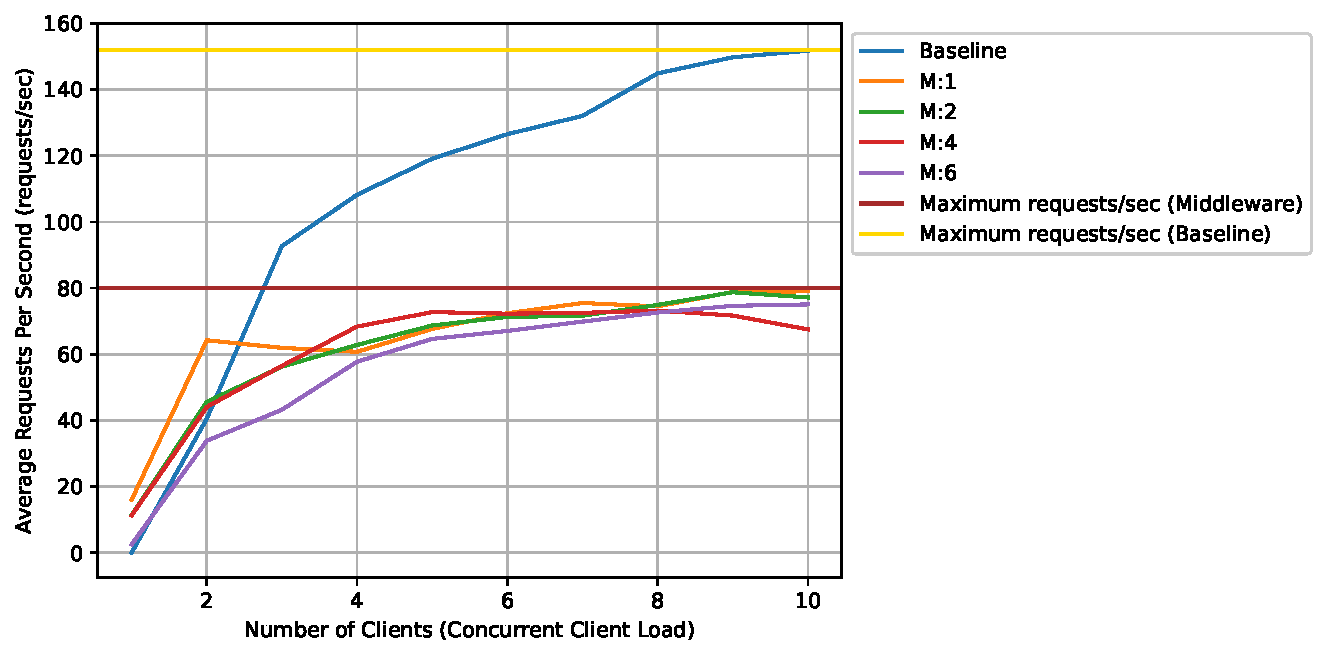
\includegraphics[width=\textwidth]{gfx/reports/throughput/average_rps_10.pdf}}{\caption{Average throughput with respect to increasing client-load ranging from 1 to 10}\label{average_rps_10}}
\end{figure}


%%%%%%%%%%%%
\subsection*{\textbf{Average Response Time}}

To measure the average response time of the middleware with different configurations, a progressively increasing client-load ranging from 1 to 50 is considered, as defined in \textbf{Test Scenario: 4} within subsection \ref{testScenario}. For the baseline, the average response time of a single Redis database connected to a single client is measured. As depicted in \cref{average_res_50}, the baseline exhibits a consistent and linear increase of the average response time, with the growing number of concurrent clients. The average response time begins at approximately 11.88 milliseconds (ms) for 1 client and peaks at around 94.48 ms for 50 concurrent clients, executing all operations ($set$, $get$, $get$-$range$, $delete$) with $Dataset_{1}$ and $Dataset_{2}$, as defined in subsection \ref{workloadBenchmark}. The observed response time for the baseline shows a linear growth of about 1.70 ms. \\

\noindent For assessing the average response time of the middleware as perceived by the connected client, it is essential to consider factors, directly or indirectly influencing the response time. These factors include:
\begin{itemize}
\item[-]	Processing time of the middleware (Service Time)
\item[-]	Internal response time of the associated Redis databases within the middleware
\item[-]	Waiting time of the middleware for the corresponding response (Wait Time)
\item[-]	Network latencies, i.e., the time delays caused by the network between the client and the middleware, as well as between the middleware and the associated Redis databases.
\end{itemize}

\begin{figure}[H]
             \ffigbox{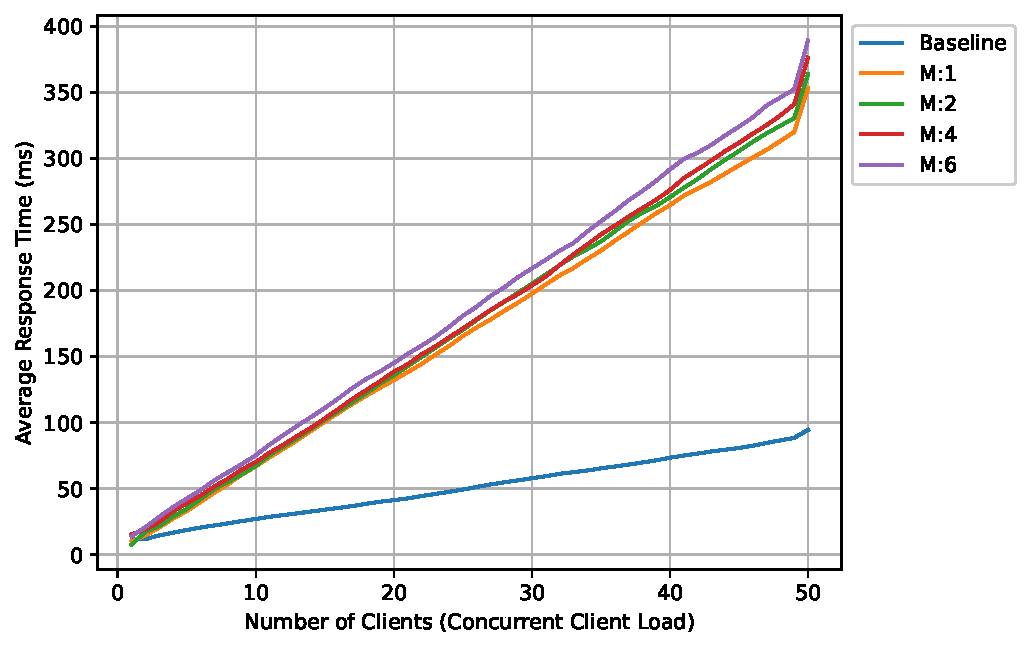
\includegraphics[width=\textwidth]{gfx/reports/response_time/avg_response_time_50.pdf}}{\caption{Average response time with respect to steadily increasing client-load from 1 to 50}\label{average_res_50}}
\end{figure}

\noindent Both network latencies and processing times are dynamic factors that change with time and scenarios, making it difficult to obtain concrete and accurate measurements. Due to these factors, the response time may include some noise and unintentional delays. Hence, the outcomes from the load-test executions should be considered approximate values. \cref{tab:response_time_average} states the observed average response times of the baseline and all the middleware configurations with constant client-load of 1, 10, and 100. 

\begin{table} [H]
\centering
\begin{tabular}{@{} lrrrrr @{}} % @{} removes white spaces
	\toprule
	 %\multirow{2}{*}{\spacedlowsmallcaps{Client-Load (N)}} & \multirow{2}{*}{\spacedlowsmallcaps{Baseline (N)}} & \multirow{2}{*}{\spacedlowsmallcaps{M:1}} &  \multirow{2}{*}{\spacedlowsmallcaps{M:2}} &  \multirow{2}{*}{\spacedlowsmallcaps{M:4}} &  \multirow{2}{*}{\spacedlowsmallcaps{M:6}} \\ 
	Client-load	&	Baseline	&	M:1	&	M:2  &		M:4  & 	M:6  \\
	\midrule
	1 &	10.46 ms	&	15.10 ms	&	16.47 ms	&	17.62 ms	&	18.63 ms \\
	10 &	40.33 ms	&	125.75 ms	&	128.57 ms &	134.42 ms	&	135.63 ms \\
	100 &	327.32 ms &	1297.37 ms &	 1353.55 ms &	1360.46 ms & 1372.55 ms \\
	\bottomrule
\end{tabular}
\caption{Observed average response time of the middleware and the baseline with different client-load}
\label{tab:response_time_average}
\end{table}

\noindent Considering the saturation point of 10 client-load, as per the evaluation of throughput of the baseline and the middleware, the observed response time behavior concerning the number of concurrent clients in the system is represented in \cref{average_res_10}.

\begin{figure}[H]
             \ffigbox{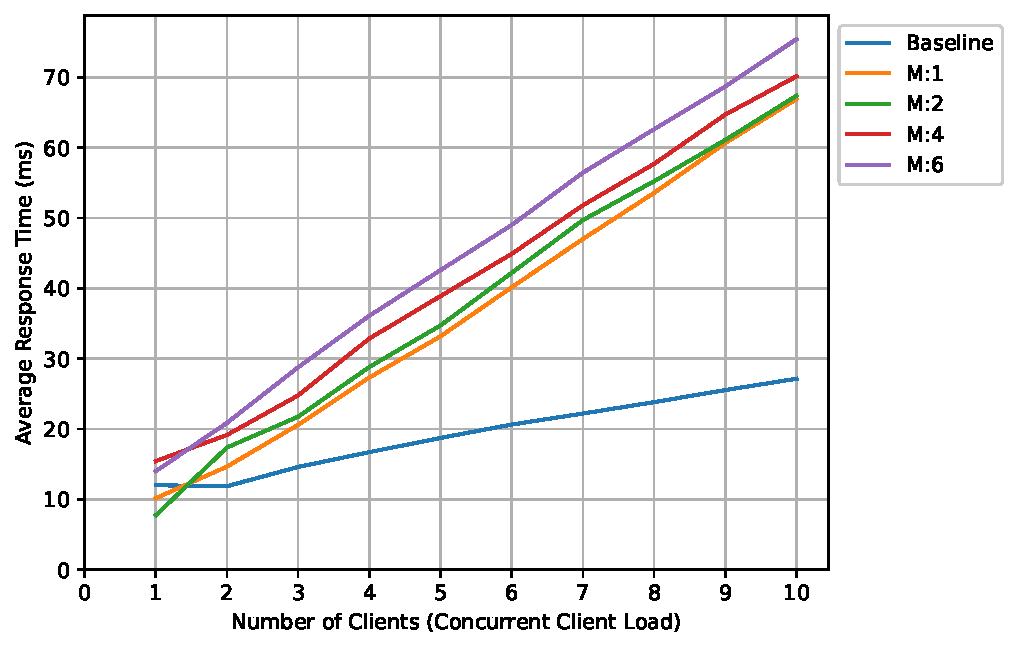
\includegraphics[width=\textwidth]{gfx/reports/response_time/avg_response_time_10.pdf}}{\caption{Average response time with respect to steadily increasing client-load from 1 to 10}\label{average_res_10}}
\end{figure}

\noindent Based on the evaluation, it can be concluded that the average response time of both the baseline and the middleware for all configurations increases linearly. The observed linear growth in the middleware’s response time with increasing number of concurrent clients from 1 to 10 is given in \cref{tab:linear_growth_rate}.

\begin{table} [H]
\centering
\begin{tabular}{@{} ccc @{}} % @{} removes white spaces
	\toprule
	 %\tableheadline{Middleware Configurations} & & \tableheadline{Linear Growth Rate (Response Time)} \\
	 Middleware Configurations & & Linear Growth Rate (Response Time) \\
	\midrule
	M:1 &	&	 $\approx$ 6.66 ms \\
	M:2 &	&	 $\approx$ 6.37 ms \\
	M:4 &	&	 $\approx$ 6.10 ms \\
	M:6 &	&	 $\approx$ 6.23 ms \\
	\bottomrule
\end{tabular}
\caption{Linear growth rate of the average response time observed in different middleware configurations}
\label{tab:linear_growth_rate}
\end{table}

\noindent To obtain meaningful comparisons between the middleware and the baseline, set and get operations involving single and multiple key-value pairs are thoroughly analyzed, focusing on a single client connected to one middleware instance, as illustrated in \cref{set_get_m1}, \cref{set_get_m2}, \cref{set_get_m4}, and \cref{set_get_m6}. The middleware with 1 Redis database (M:1), providing an interface to a single client, has an average response time of approximately 3.89 ms for storing or setting 1 key-value pair in the database, whereas it has an average response time of around 4.01 ms for retrieving the 1 key-value pair from the database. In the case of 1000 key-value pairs, M:1 has an average response time of around 41.85 ms for setting all the key-value pairs and 38.36 ms for retrieving all of them. The average response time observed in the baseline for setting 1 key-value pair is around 1.89 ms, while for getting 1 key-value pair, it is around 2.11 ms. Meanwhile, for the 1000 key-value pairs, the average response times for setting and getting multiple key-value pairs are around 24.03 ms and 21.91 ms, respectively, which is nearly half of the average response time observed from M:1. \\

\begin{figure}[H]
	\begin{floatrow}
             \ffigbox{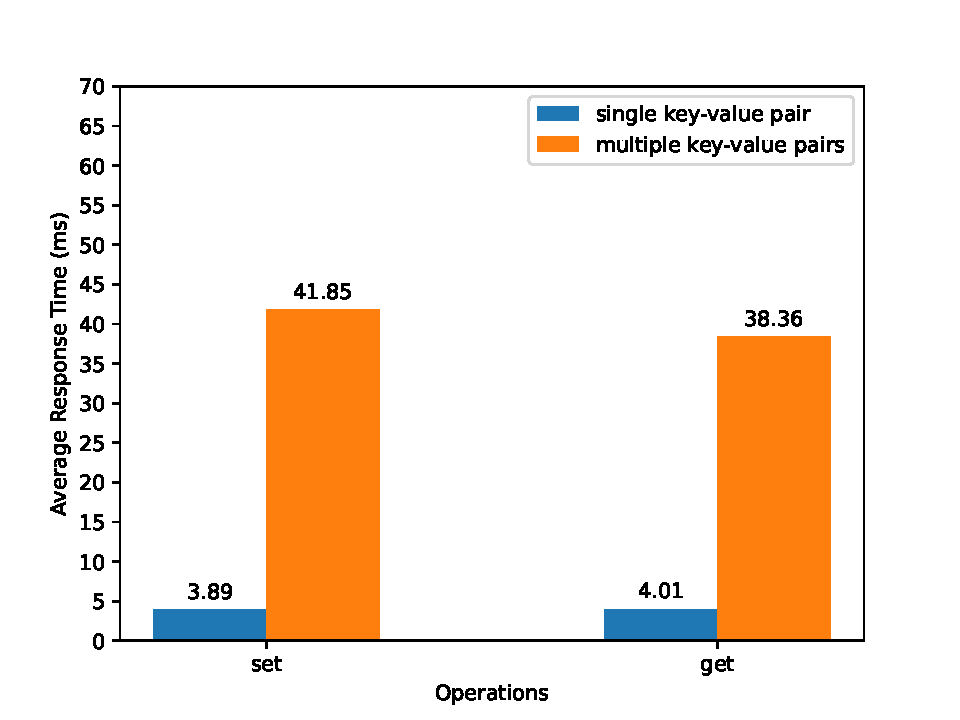
\includegraphics[scale = 0.5]{gfx/reports/response_time/set_get/set_get_1_Client_M-1.pdf}}{\caption{Set and Get operations with M:1}\label{set_get_m1}}
             \ffigbox{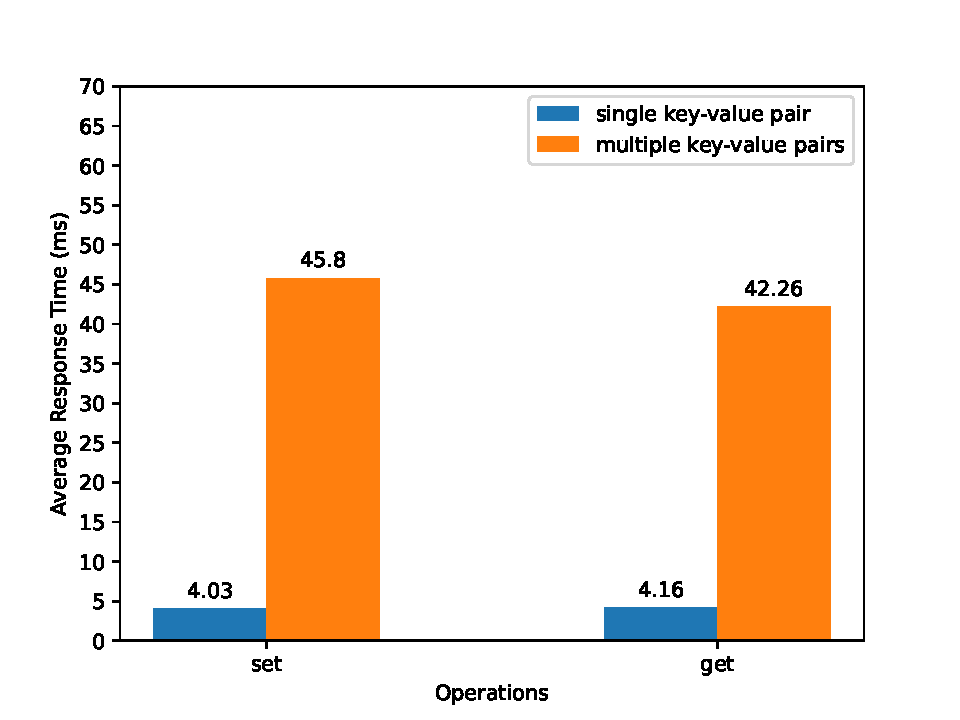
\includegraphics[scale = 0.5]{gfx/reports/response_time/set_get/set_get_1_Client_M-2.pdf}}{\caption{Set and Get operations with M:2}\label{set_get_m2}}
	\end{floatrow}
\end{figure}
\begin{figure}[H]
	\begin{floatrow}
             \ffigbox{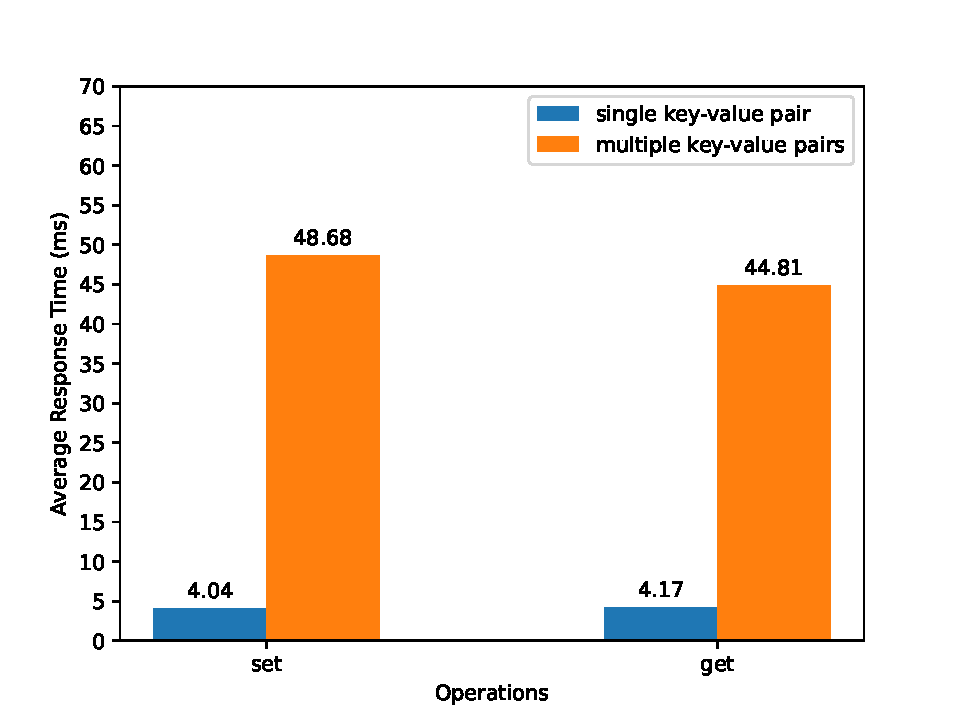
\includegraphics[scale = 0.5]{gfx/reports/response_time/set_get/set_get_1_Client_M-4.pdf}}{\caption{Set and Get operations with M:4}\label{set_get_m4}}
             \ffigbox{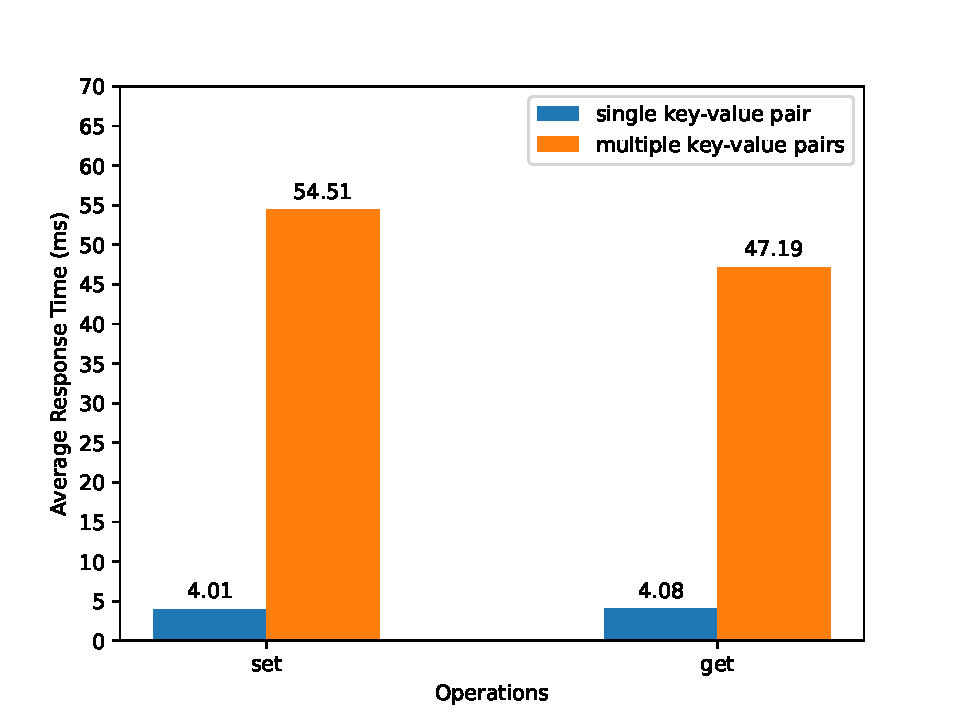
\includegraphics[scale = 0.5]{gfx/reports/response_time/set_get/set_get_1_Client_M-6.pdf}}{\caption{Set and Get operations with M:6}\label{set_get_m6}}
	\end{floatrow}
\end{figure}

\noindent Comparing the observed response times reveals a significant difference between setting and getting 1 key-value pair versus 1000 key-value pairs. This disparity can be attributed to the workload. In the baseline, setting and retrieving 1 key-value pair occurs sequentially, while for 1000 key-value pairs, a pipeline is created to queue all requests and a single bulk operation request is sent. In the middleware, 1 key-value pair is not sharded and is directly stored or fetched from the associated Redis database, whereas for 1000 key-value pairs, sharding is performed, which introduces processing overhead. Additionally, factors such as network latencies and communication overhead negatively impact the middleware's response time. \\

\begin{figure}[H]
             \ffigbox{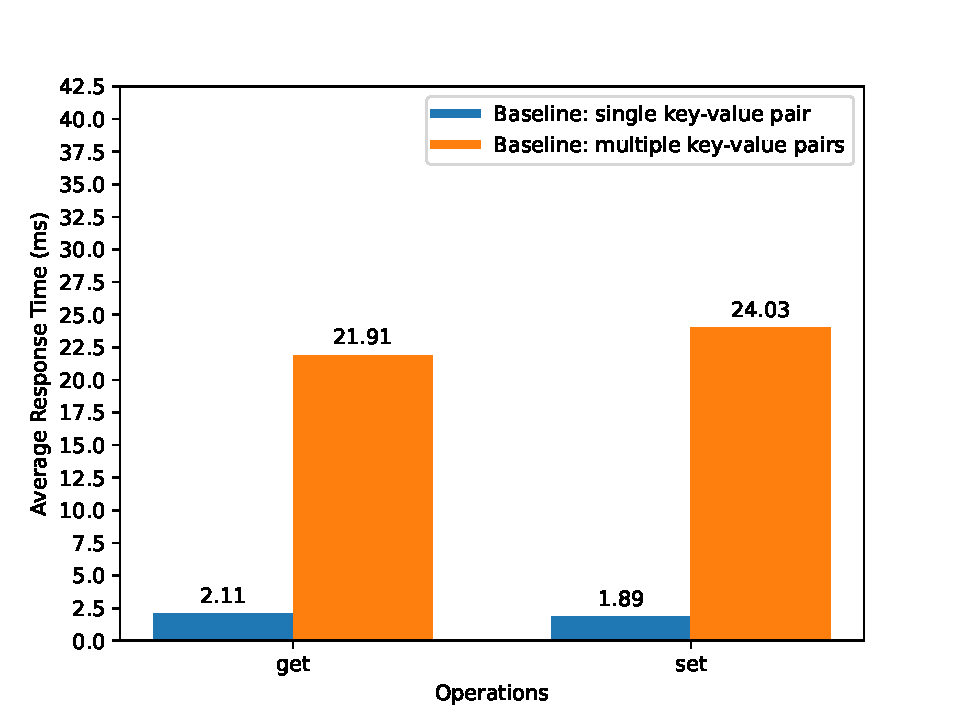
\includegraphics[scale = 0.5]{gfx/reports/response_time/set_get/set_get_baseline.pdf}}{\caption{Set and Get operations with Baseline}\label{set_get_baseline}}
\end{figure}
 
\noindent The difference between setting and getting 1 key-value pair in the baseline and the middleware should not be significant; however, the results indicate otherwise. This discrepancy can be attributed to the middleware introducing additional communication entities, which further increases processing overhead unless the middleware is carefully designed with concurrency features and optimized utilization of computing resources. A bottleneck also arises when using a single middleware instance to communicate with clients and all associated Redis databases. This is another reason for the slight degradation in the middleware's response time when more Redis databases are added. As more Redis databases are connected to a single middleware instance, the average response time also increases by 1 to 6 ms, as shown in \cref{set_get_m2} for M:2, \cref{set_get_m4} for M:4, and \cref{set_get_m6} for M:6. \\

\noindent For a more fine-grained evaluation, the average response time of the middleware is divided into two components:
\begin{itemize}
\item[-]	Internal response time from the connected databases within the middleware ($Internal\:DB$-$RT$)
\item[-]	$Service\:Time$ and $Wait\:Time$ for requests and responses
\end{itemize}
For the simplification of performance analysis, the average response time is considered as the total response time observed with the middleware. With this approach, the total $Response\:Time$ ($RT$) can be derived as: \\ 

$Total\:RT$ $\approx$ $Internal\:DB$-$RT$ + ($Service\:Time$ and $Wait\:Time$ ) \\

\noindent \cref{overview_rt} provides detailed information about the total response time, internal response time within the middleware, and the waiting and processing time of the middleware with various configurations. As observed in \cref{set_get_baseline} and the results outlined in \cref{overview_rt}, the $Internal\:DB$-$RT$ for set and get operations for a single key-value pair is smaller than the observed response time in the baseline. This difference can be attributed to the connection setup time of the Redis database in the baseline, while in the middleware, the connection to the Redis database is already established during the middleware's startup. However, the $Total\:RT$ of the middleware is slower than the baseline due to the $Service\:Time$ of the middleware for the requests and the $Wait\:Time$ of the responses from the associated databases. Consequently, this result indicates that the baseline is almost twice as responsive as the M:1 configuration. \\

\begin{table} [H]
\centering
\begin{tabular}{@{}llccr@{}} 
\toprule
     \multirow{2}{*}{Middleware} & \multirow{2}{*}{Requests} & \multirow{2}{*}{Total RT} & Internal  & Service Time and  \\
      & & & DB-RT & Wait Time  \\
    \midrule
    \multirow{7}{*}{M:1} & set\textunderscore single  & 3.9896 & 1.7717 & 2.2179  \\
    &	set\textunderscore multiple  & 41.8467  & 16.9528 & 24.8939  \\
    &	get\textunderscore single  & 4.0148  & 0.5548 & 3.4600  \\
    &	get\textunderscore multiple  & 38.3633 & 11.2019 & 27.1615    \\ 
    &	get\textunderscore range  & 7.9164   & 1.6844 & 6.2319 \\
    &	del\textunderscore single  & 4.0209 & 0.3221 & 3.6988  \\
    &	del\textunderscore multiple  & 6.9168  & 1.6909 & 5.2259   \\ \midrule

     \multirow{7}{*}{M:2} & set\textunderscore single  & 4.0261 & 1.7490 & 2.277  \\
    &	set\textunderscore multiple  & 45.7991  & 19.1634 & 26.6358   \\
    &	get\textunderscore single  & 4.1628  & 0.5383 & 3.6245  \\
    &	get\textunderscore multiple  & 42.259  & 12.4283 & 29.8307     \\ 
    &	get\textunderscore range  & 8.8411   & 2.7823 & 6.0588 \\
    &	del\textunderscore single  & 4.1352  & 0.3929 & 3.7423   \\
    &	del\textunderscore multiple  & 7.6919  & 2.1648 & 5.5271    \\ \midrule
    
     \multirow{7}{*}{M:4} & set\textunderscore single  & 4.0353		& 	1.7843		&	2.2510 \\
    &	set\textunderscore multiple  &  48.6758	&	20.7641	&	27.9117 \\
    &	get\textunderscore single  & 	4.1707		& 	0.4332		&	3.7375 \\
    &	get\textunderscore multiple  &		44.8088	&	 14.1521	&	30.6568 \\ 
    &	get\textunderscore range  & 	 9.8087		&	 3.6182		&	6.1904 \\
    &	del\textunderscore single  & 	4.0891		& 	0.3047		&	3.7844 \\
    &	del\textunderscore multiple  & 8.6419		& 	3.221		& 	5.4208 \\ \midrule

     \multirow{7}{*}{M:6} & set\textunderscore single  &	4.0051 & 	1.7750 	& 2.2301		\\
    &	set\textunderscore multiple  &		54.5115 	& 	22.8808 	& 	31.6307		\\
    &	get\textunderscore single &	4.0775 	& 	0.4649 	& 	3.6126			\\
    &	get\textunderscore multiple  &		47.1893 	& 15.4793 	& 	31.7100		\\
    &	get\textunderscore range   &	11.2084	 & 	3.7737 	& 	7.4347		\\
    &	del\textunderscore single  &	4.1074 	& 	0.1915 	&	 3.9160		\\
    &	del\textunderscore multiple  &		9.8391 	& 	3.9923 	& 	5.8468		\\
 	\bottomrule
\end{tabular}
\caption[Comprehensive overview of average response time and processing overhead of middleware]{Comprehensive overview of average response time and processing overhead of the system with a single client connected to the middleware}
\label{overview_rt}
\end{table}

%%%%%%%%%%%%
\section{Data Distribution Analysis}
\label{dataDistribution}

This subsection provides a brief evaluation of the middleware's consistent hash sharding approach in achieving efficient and uniform data distribution among Redis databases. \\

\noindent The middleware employs consistent hashing for sharding large datasets, which ensures that the load is evenly distributed among the database nodes. Moreover, this approach guarantees that adding a new database node does not necessitate rehashing all data items \cite{1372064}. However, the addition and removal of database nodes in the system are beyond the scope of this thesis. In this section, a synthetic workload of 100 and 1000 key-value pairs as mentioned in the subsection \ref{workloadBenchmark}, is utilized to assess the data distribution across Redis databases using the consistent hashing approach. \\

\noindent The test executions employ middleware configurations, M:2 (2 shards), M:4 (4 shards), and M:6 (6 shards), as detailed in the subsection \ref{config}. The middleware with 1 Redis database (1 shard), i.e., M:1 is excluded from this test, as data distribution is not applicable with a 1 shard and all data is stored in 1 Redis database node. The ideal data distribution across all Redis databases would involve each database having an equal number of key-value pairs. However, achieving perfect data distribution and maintaining an equal number of key-value pairs in each Redis database is challenging. \\

\noindent In the middleware connected to 2 Redis databases (M:2), ideal data distribution for 100 key-value pairs would involve splitting them evenly, with 50 allocated to each Redis database. Similarly, for 1000 key-value pairs, each of the 2 Redis databases should store 500 key-value pairs. The middleware distributes 100 key-value pairs as follows: 61 in the first Redis database and 39 in the second. Although not perfect, the difference of these 22 key-value pairs is not substantial. Compared to the ideal distribution of 50 key-value pairs each, the first Redis database stores 11 more, while the second stores 11 fewer. For 1000 key-value pairs, the distribution results in 526 stored in the first Redis database and 474 in the second. These findings are illustrated in \cref{data_2_db}. \\

\noindent The middleware with 4 Redis databases (M:4) distributes the 100 key-value pairs as follows: 32 in the first Redis database node, 23 in the second, 30 in the third, and 15 in the fourth. Ideally, each database node should have 25 key-value pairs. However, the current data distribution ensures that no database experiences a data hotspot, as a maximum of only 32 key-value pairs are allocated to a single Redis database. This data distribution trend continues for 1000 key-value pairs, where a maximum of 291 key-value pairs are assigned to a single Redis database. The detailed result of data distribution in M:4 is illustrated in \cref{data_4_db}. \\

\noindent Data distribution in the middleware with 6 Redis databases (M:6) appears more uniform compared to previous middleware configurations. For 100 key-value pairs, the data is divided among the 6 databases or shards, with an ideal scenario of approximately 16 to 17 key-value pairs in a single database. For 1000 key-value pairs, the ideal distribution would be 166 to 167 key-value pairs per database. \cref{data_6_db} presents the optimal data distribution results achieved by M:6.

\begin{figure} [H]
    \centering
    \begin{subfigure}[b]{0.45\textwidth}
    \centering
    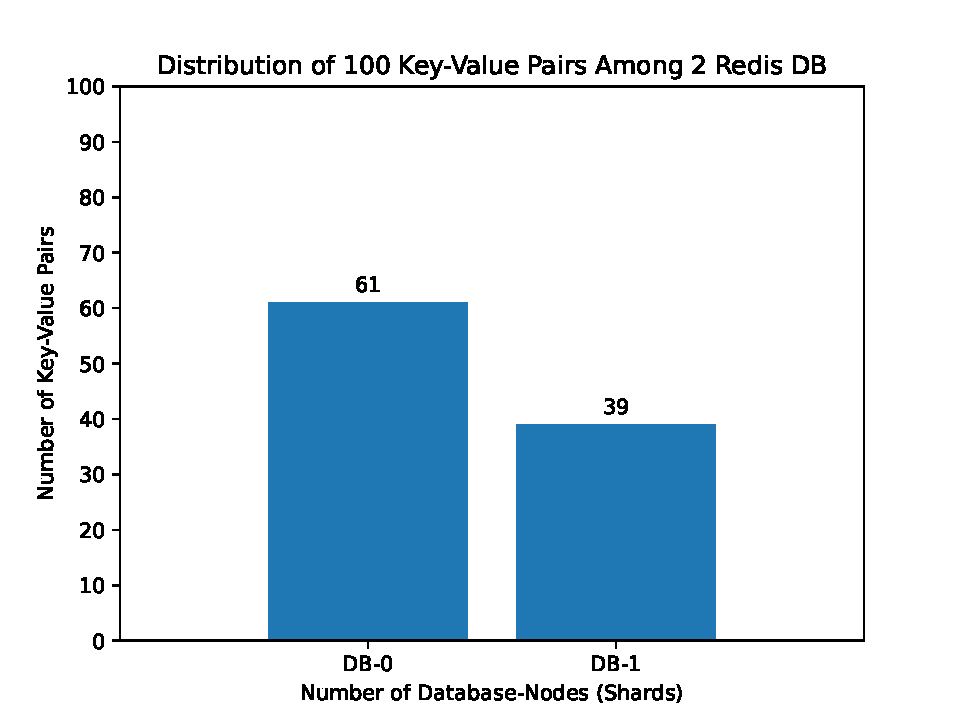
\includegraphics[width=\textwidth]{gfx/reports/data_distribution/2_DB/distribution-100.pdf}
    \end{subfigure}
    \begin{subfigure}[b]{0.45\textwidth}
    \centering
    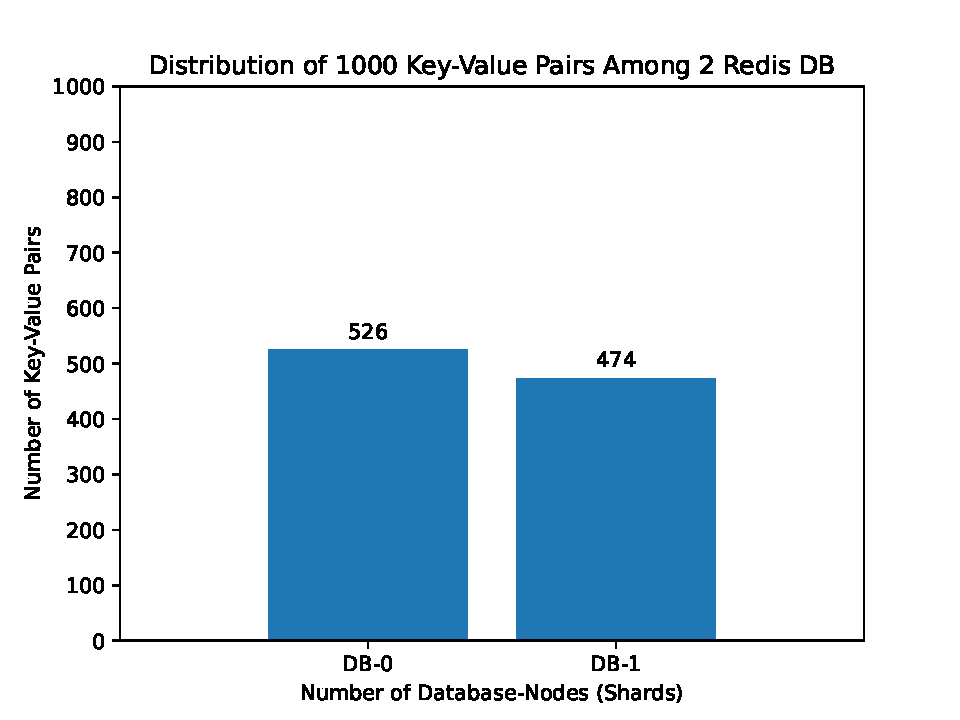
\includegraphics[width=\textwidth]{gfx/reports/data_distribution/2_DB/distribution-1000.pdf}
    \end{subfigure}
    \caption{Data distribution among 2 Redis databases (2 Shards)}
    \label{data_2_db}
\end{figure}

\begin{figure} [H]
    \centering
    \begin{subfigure}[b]{0.45\textwidth}
    \centering
    
\includegraphics[width=\textwidth]{gfx/reports/data_distribution/4_DB/distribution-100.pdf}
    \end{subfigure}
    \begin{subfigure}[b]{0.45\textwidth}
    \centering
    
\includegraphics[width=\textwidth]{gfx/reports/data_distribution/4_DB/distribution-1000.pdf}
    \end{subfigure}
    \caption{Data distribution among 4 Redis databases (4 Shards)}
    \label{data_4_db}
\end{figure}

\begin{figure} [H]
    \centering
    \begin{subfigure}[b]{0.45\textwidth}
    \centering
    
\includegraphics[width=\textwidth]{gfx/reports/data_distribution/6_DB/distribution-100.pdf}
    \end{subfigure}
    \begin{subfigure}[b]{0.45\textwidth}
    \centering
    
\includegraphics[width=\textwidth]{gfx/reports/data_distribution/6_DB/distribution-1000.pdf}
    \end{subfigure}
    \caption{Data distribution among 6 Redis databases (6 Shards)}
    \label{data_6_db}
\end{figure}







